%----------
%	CONFIGURACIÓN DEL DOCUMENTO
%----------
\documentclass[12pt]{report} %fuente a 12pt
% MÁRGENES: 2,5 cm sup. e inf.; 3 cm izdo. y dcho.
\usepackage[
  a4paper,
  vmargin=2.5cm,
  hmargin=3cm
]{geometry}

% INTERLINEADO: Estrecho (6 ptos./interlineado 1,15) o Moderado (6 ptos./interlineado 1,5)
\renewcommand{\baselinestretch}{1.15}
\parskip=6pt

% DEFINICIÓN DE COLORES para portada y listados de código
\usepackage[table]{xcolor}
\definecolor{azulUC3M}{RGB}{0,0,102}
\definecolor{gray97}{gray}{.97}
\definecolor{gray75}{gray}{.75}
\definecolor{gray45}{gray}{.45}

\usepackage[a-1b]{pdfx}
\usepackage{hyperref}

\hypersetup{colorlinks=true,
	linkcolor=black, % enlaces a partes del documento (p.e. índice) en color negro
	urlcolor=blue} % enlaces a recursos fuera del documento en azul

% EXPRESIONES MATEMATICAS
\usepackage{amsmath,amssymb,amsfonts,amsthm}

\usepackage{txfonts}
\usepackage[T1]{fontenc}
\usepackage[utf8]{inputenc}

\usepackage[spanish, es-tabla]{babel}
\usepackage[babel, spanish=spanish]{csquotes}
\AtBeginEnvironment{quote}{\small}

% diseño de PIE DE PÁGINA
\usepackage{fancyhdr}
\pagestyle{fancy}
\fancyhf{}
\renewcommand{\headrulewidth}{0pt}
\rfoot{\thepage}
\fancypagestyle{plain}{\pagestyle{fancy}}

% DISEÑO DE LOS TÍTULOS de las partes del trabajo (capítulos y epígrafes o subcapítulos)
\usepackage{titlesec}
\usepackage{titletoc}
\titleformat{\chapter}[block]
{\large\bfseries\filcenter}
{\thechapter.}
{5pt}
{\MakeUppercase}
{}
\titlespacing{\chapter}{0pt}{0pt}{*3}
\titlecontents{chapter}
[0pt]
{}
{\contentsmargin{0pt}\thecontentslabel.\enspace\uppercase}
{\contentsmargin{0pt}\uppercase}
{\titlerule*[.7pc]{.}\contentspage}

\titleformat{\section}
{\bfseries}
{\thesection.}
{5pt}
{}
\titlecontents{section}
[5pt]
{}
{\contentsmargin{0pt}\thecontentslabel.\enspace}
{\contentsmargin{0pt}}
{\titlerule*[.7pc]{.}\contentspage}

\titleformat{\subsection}
{\normalsize\bfseries}
{\thesubsection.}
{5pt}
{}
\titlecontents{subsection}
[10pt]
{}
{\contentsmargin{0pt}
	\thecontentslabel.\enspace}
{\contentsmargin{0pt}}
{\titlerule*[.7pc]{.}\contentspage}

\usepackage{multirow} % permite combinar celdas
\usepackage{caption} % para personalizar el título de tablas y figuras
\usepackage{floatrow} % utilizamos este paquete y sus macros \ttabbox y \ffigbox para alinear los nombres de tablas y figuras de acuerdo con el estilo definido. Para su uso ver archivo de ejemplo
\usepackage{array} % con este paquete podemos definir en la siguiente línea un nuevo tipo de columna para tablas: ancho personalizado y contenido centrado
\newcolumntype{P}[1]{>{\centering\arraybackslash}p{#1}}
\DeclareCaptionFormat{upper}{#1#2\uppercase{#3}\par}

% Diseño de tabla para ingeniería
\captionsetup[table]{
	format=upper,
	name=TABLA,
	justification=centering,
	labelsep=period,
	width=.75\linewidth,
	labelfont=small,
	font=small,
}

\usepackage{graphicx}
\graphicspath{{imagenes/}} %ruta a la carpeta de imágenes

% Diseño de figuras para ingeniería
\captionsetup[figure]{
	format=hang,
	name=Fig.,
	singlelinecheck=off,
	labelsep=period,
	labelfont=small,
	font=small
}

% NOTAS A PIE DE PÁGINA
\usepackage{chngcntr} %para numeración contínua de las notas al pie
\counterwithout{footnote}{chapter}

% LISTADOS DE CÓDIGO
% soporte y estilo para listados de código. Más información en https://es.wikibooks.org/wiki/Manual_de_LaTeX/Listados_de_código/Listados_con_listings
\usepackage{listings}

% definimos un estilo de listings
\lstdefinestyle{estilo}{ frame=Ltb,
	framerule=0pt,
	aboveskip=0.5cm,
	framextopmargin=3pt,
	framexbottommargin=3pt,
	framexleftmargin=0.4cm,
	framesep=0pt,
	rulesep=.4pt,
	backgroundcolor=\color{gray97},
	rulesepcolor=\color{black},
	%
	basicstyle=\ttfamily\footnotesize,
	keywordstyle=\bfseries,
	stringstyle=\ttfamily,
	showstringspaces = false,
	commentstyle=\color{gray45},
	%
	numbers=left,
	numbersep=15pt,
	numberstyle=\tiny,
	numberfirstline = false,
	breaklines=true,
	xleftmargin=\parindent
}

\captionsetup[lstlisting]{font=small, labelsep=period}
% fijamos el estilo a utilizar
\lstset{style=estilo}
\renewcommand{\lstlistingname}{\uppercase{Código}}


%-------------
%	DOCUMENTO
%-------------

\begin{document}
\pagenumbering{roman} % Se utilizan cifras romanas en la numeración de las páginas previas al cuerpo del trabajo

%----------
%	PORTADA
%----------
\begin{titlepage}
	\begin{sffamily}
	\color{azulUC3M}
	\begin{center}
		\begin{figure}[H] %incluimos el logotipo de la Universidad
			\makebox[\textwidth][c]{
\includegraphics[width=16cm]{Portada_Logo.png}}
		\end{figure}
		\vspace{2.5cm}
		\begin{Large}
			Máster en Ingeniería Informática\\
			2020 - 2021\\
			\vspace{2cm}
			\textsl{Computación de Altas Prestaciones}
			\bigskip

		\end{Large}
		 	{\Huge ``Paralelización de código con OpenMP + MPI''}\\
		 	\vspace*{0.5cm}
	 		\rule{10.5cm}{0.1mm}\\
			\vspace*{0.9cm}
			{\LARGE Carlos Vigil González}\\
            {\LARGE David Gil López}\\
			{\LARGE Daniel Alejandro Rodríguez López}\\
			\vspace*{1cm}
	\end{center}
	\vfill
	\color{black}
	% 
\includegraphics[width=4.2cm]{imagenes/creativecommons.png}\\ %incluimos el logotipo de creativecommons
	% \emph{[Incluir en el caso del interés en su publicación en el archivo abierto]}\\  % BORRAR ESTA LÍNEA
	% Esta obra se encuentra sujeta a la licencia Creative Commons \textbf{Reconocimiento - No Comercial - Sin Obra Derivada}
	\end{sffamily}
\end{titlepage}

%--
% Índice general
%-
\tableofcontents
\thispagestyle{fancy}

%--
% Índice de figuras. Si no se incluyen, comenta las líneas siguientes
%-
\listoffigures
\thispagestyle{fancy}

%--
% Índice de tablas. Si no se incluyen, comenta las líneas siguientes
%-
\listoftables
\thispagestyle{fancy}

%----------
%	TRABAJO
%----------
\clearpage
\pagenumbering{arabic} % numeración con múmeros arábigos para el resto de la publicación

\chapter{Introducción}
\label{chap:Intro}

La presente memoria explica los pasos seguidos, experimentacón y resultados obtenidos durante la paralelización del código de equalización de histograma entregado inicialmente. Pero antes de entrar en resultados, conviene explicar en qué consiste una equalización de histograma.

De forma simplista, una equalización de histograma consiste en estirar el rango de valores en una imagen para aplanar su histograma de valores.

\begin{figure}[H]
    \makebox[\textwidth][c]{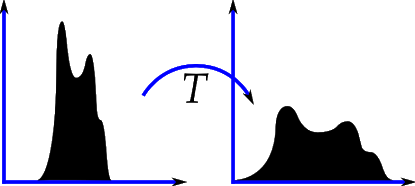
\includegraphics[width=12cm]{histogram_equalization.png}}
    \caption{Ejemplo de Equalización de Histograma}
    \label{fig:hist_eq}
\end{figure}

De forma un poco más técnica, una equalización de histograma distribuye los valores de color en una imagen de forma que todos se encuentran presentes de forma equitativa dentro de la imagen, como se puede apreciar en la \autoref{fig:hist_eq}

Para calcular estos histogramas se debe recorrer la imagen multiples veces, tanto para calcular los valores iniciales como para establecer los valores finales, por lo tanto hemos orientado nuestros esfuerzos con OpenMP(PODRÍAMOS METER REFERENCIA A LA WEB DE OPENMP, PERO NO SE USAR LA BIBLIOGRAFÍA EN LATEX XD) en optimizar estas iteraciones sobre la imagen, mientras que con MPI(MISMO QUE CON OPENMP) nos hemos centrado en el reparto de fragmentos de la imagen entre distintos procesos para reducir el número de iteraciones.

No obstante para poder obtener un análisis más completo de las distintas alternativas y \textit{speed-ups} posibles, se han realizado 3 versiones distintas de paralelización: \nameref{chap:OpenMP}, \nameref{chap:MPI} y \nameref{chap:OpenMP+MPI}. De igual forma, para poder comparar los resultados de forma fiable, se ha utilizado las mismas imágenes de prueba, entorno de ejecución (guernika) y número de ejecuciones.

\section{Análisis}

CARLOS DICE QUE: ESTO CARLOS

Aquí creo que habría que comentar de qué formas hemos visto que es posible paralelizar el código inicial y que partes hacerlas por OpenMP y otras por MPI

\subsection{Speed up teóricos}

Antes de empezar a realizar ningún cambio sobre el código, con el objetivo de conocer qué mejoras podemos esperar a la hora de paralelizarlo, se ha calculado un \textit{speed up} teórico para la \nameref{sec:Amdahl} y para la \nameref{sec:Gustafson}.

\subsubsection{Ley de Amdahl}
\label{sec:Amdahl}

La Ley de Amdahl nos permite dado un programa con carga fija, el \textit{speed up} máximo que podríamos alcanzar

\[ S = \frac{1}{(1 - P) + \frac{P}{N}} \]

Siendo S el \textit{speed up}, P la fracción paralela de código y N el número de núcleos entre los que la dividimos.

%total = 19+7+59+17+116+70
%paralelo = 7+17+70
De esta forma, en el código original tenemos 288 líneas de código, de las cuales hemos identificado 94 como parelizables, dándo lugar a una $P = 0.32638$.

\begin{figure}[H]
    \makebox[\textwidth][c]{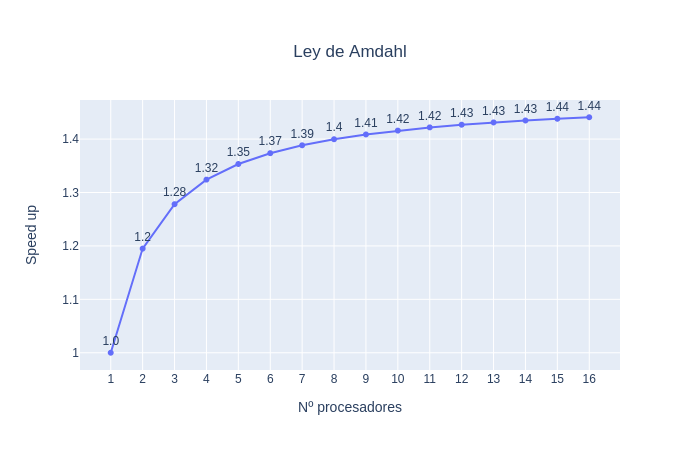
\includegraphics[width=14cm]{amdahl.png}}
    \caption{Ley de Amdahl con distinto N}
    \label{fig:fig_amdahl}
\end{figure}

Como se puede observar el \textit{speed up} se empieza a detener a partir de los 8 procesadores, ya que de un \textit{speed up} de 1.4 pasamos a 1.44 con 16 procesadores, por lo que no tiene mucho sentido aumentar el número de procesadores ya que la ganancia sería mínima.

\subsubsection{Ley de Gustafson}
\label{sec:Gustafson}

\[ S = P - \alpha \cdot (P - 1)\]

Siendo P el número de procesadores y $\alpha$ la parte de código no paralelizable.


\chapter{OpenMP}
\label{chap:OpenMP}

Como se comentó brevemente en la \nameref{chap:Intro} nuestro objetivo con OpenMP en la versión combinada se centrará en optimizar las iteraciones de cálculos sobre las imágenes. De igual forma, en esta versión que usa únicamente OpenMP también nos hemos centrado en lo mismo, ya que resulta, además de mucho más sencillo, igual o más óptimo repartir la carga de trabajo en cada una de las iteraciones, que dividir la imagen al inicio y luego juntar todos los resultados cada vez que sea necesario, ya que existen pasos intermedios que deben ser calculados con toda la imagen.


\section{Paralelización}

Dada la premisa anterior, dividir la imagen desde el comienzo sería perjudicial para el rendimiento ya que habría que estar haciendo varios \texttt{join} que nos podríamos evitar si paralelizamos los bucles en vez de particionar la imagen desde el comienzo.

Sin embargo no hemos paralelizado todos los bucles existentes en el código, ya que aquellos con pocas iteraciones se verían afectados negativamente al parelelizar por el \textit{overhead} que introducimos con OpenMP. Estos bucles que han sido ignorados son aquellos que dependen de la variable \texttt{nbr\_bin}, se debe a que sus valores van desde 0 hasta 255, que son todos los valores posibles en la escala de grises. Al ser tan pocas iteraciones y además tratarse de bucles con poca carga computacional no compensa paralelizarlos. Por otro lado, los bucles que sí han sido paralelizados y compensa notablemente son aquellos que dependen del tamaño de la imagen, ya que incluso una imagen pequeña de 200x200 se transforma en 40000 iteraciones.


\section{Experimentación}

La experimentación se ha realizado usando la imagen proporcionada de ejemplo (11472 x 6429 píxeles), usando el entorno de guernika (6 núcleos físicos y otros 6 virtuales, 12 en total a 3,4GHz) y repitiendo durante 100 ejecuciones.

En los resultados se pueden observar los tiempos obtenidos con el código original y los nuevos tiempos de esta versión.

\chapter{MPI}
\label{chap:MPI}

Explicar nuestro objetivo con MPI y cómo hemos paralelizado cosas

\section{Paralelización}

\section{Experimentación}

La experimentación se ha realizado usando la imagen proporcionada de ejemplo (11472 x 6429 píxeles), usando el entorno de guernika (6 núcleos físicos y otros 6 virtuales, 12 en total a 3,4GHz) y repitiendo durante 100 ejecuciones.

En los resultados se pueden observar los tiempos obtenidos con el código original y los nuevos tiempos de esta versión.

\chapter{OpenMP + MPI}
\label{chap:OpenMP+MPI}
Explicar "conclusiones" o yuqse sobre porqué en base a lo anterior hemos decidido hacer el OpenMP+MPI final, quizás no es exáctamente igual que simplemente juntar lo anterior

\section{Paralelización}

\section{Experimentación}

La experimentación se ha realizado usando la imagen proporcionada de ejemplo (11472 x 6429 píxeles), usando el entorno de guernika (6 núcleos físicos y otros 6 virtuales, 12 en total a 3,4GHz) y repitiendo durante 100 ejecuciones.

En los resultados se pueden observar los tiempos obtenidos con el código original y los nuevos tiempos de esta versión.

\chapter{Conclusiones}

Buah colega, hemos aprendido tope mazo

\end{document}
